% A good introduction to latex can be found here:
%    http://www.cse.ohio-state.edu/~hank/latex/lshort141.pdf

\documentclass[9.5pt]{extarticle}

\usepackage{full page}  % make the margins somewhat smaller than the default
\usepackage{graphicx}
\usepackage{amsmath}
\usepackage{indentfirst}
\usepackage{color}
\usepackage{cite}
\usepackage{wasysym}
\usepackage{amssymb}
\usepackage{multirow}
\usepackage{float}
\usepackage{lscape}
\usepackage{alltt} 
\usepackage{listings}
\usepackage{booktabs}
\usepackage{mathtools}
\usepackage{fancyhdr}
\usepackage[table,xcdraw]{xcolor}

\DeclarePairedDelimiter{\ceil}{\lceil}{\rceil}
\DeclarePairedDelimiter{\floor}{\lfloor}{\rfloor}

\definecolor{dkgreen}{rgb}{0,0.6,0}
\definecolor{gray}{rgb}{0.5,0.5,0.5}
\definecolor{mauve}{rgb}{0.58,0,0.82}


\usepackage{listings}  %  needed for source code listings

\lstset{frame=tb,
  language= java,
  aboveskip=1.5mm,
  belowskip=1.5mm,
  showstringspaces=false,
  columns=flexible,
  basicstyle={\small\ttfamily},
  keywordstyle=\color{blue},
  commentstyle=\color{dkgreen},
  stringstyle=\color{mauve},
  breaklines=true,
  tabsize=2,
  numbers=left,
  stepnumber=1,    
  firstnumber=1,
  numberfirstline=true
}
       

% set the document title, author, and date here.
%  once set, the \maketitle command (within the document)
%  will display them nicely
\title{Constraint Satisfaction Problem (CSP) Assignment}
\author{Chua Zheng Fu Edrei}

\begin{document}
\maketitle

\section{Introduction}

In all of the previous assignments, we make use of problem specific heuristics to solve complex problems. Constraint Satisfaction Problem (CSP) search algorithm takes advantage of the structure of states and use a general purpose heuristic to solve problems. In this report, I will describe the implementation of a simple backtracking solver that incorporates a minimum remaining value (MRV) and least contraining value (LCV) heuristic, as well as an inference technique (FC or MAC-3 to ensure arc consistency). I will demonstrate the correctness and compare the performance of the algorithm with and without the additional heuristics on the N-Queen problem, Sudoku problem and Circuit board problem. Finally, I will describe the work by Bessiere et al on coarse-grained arc consistency algorithm.

\section{Implementation}
\subsection{CSP problem formulation}

To formulate a CSP problem, we need function that allows the addition of variable and constraints. There are a few important data structures used in the formulation. \verb`Map<Integer,Set<Integer>> D` stores the domain of each variable in the problem i.e. \verb`D.get(i)` will give the domain of the variable \verb`i`.\\
\verb`Map<Integer,Map<Integer, Set<Pair<Integer, Integer>>>> C` stores the constraint between two variables i.e. \verb`C.get(i).get(j)` will give the constraint between variable \verb`i` and \verb`j`.\verb`Set<Pair<Integer,Integer>> arc` is a set of all directed arcs and \verb`Map<Integer,Set<Integer>> graph` will allow us to access the neighbour of each variable. The function \verb`addVariable` and \verb`addConstraint` updates the value stored in the four data structures described above and the code is self-explanatory. Intrested reader should refer to the file ConstraintSatisfactionProblem.java for the implementation of the functions.

\subsection{Backtracking}

I implemented a simple backtracking solver following the pseudocode in p.215 of the textbook and the code is given in Listing 1. It is a recursive algorithm and the base case is when a solution is found (size of partial solution is same as the number of variables) or when no solution is found after looping through all possible values. It recurses if the value found is consistent with its neighbouring constraints. \verb`isConsistent` works by checking the constraint of the immediate neighbours\ of the variable \verb`var` and determine if \verb`value` and the neighbouring values stored in \verb`partialSolution` satisfy the constraints. The code for \verb`isConsistent` can be found in ConstraintSatisfactionProblem.java. Additional heuristic such as MRV (\verb`selectUnassignedVariable`) and LCV (\verb`orderDomainValues`) are implemented and the code is given in section 2.3 and 2.4. 

\begin{lstlisting}[language=java,caption={Backtracking}]
	private Map<Integer, Integer> backtracking(Map<Integer, Integer> partialSolution) {
        if(partialSolution.size() == D.size()){
            return partialSolution;
        }
        int var = selectUnassignedVariable(partialSolution);

        for(int value: orderDomainValues(var, partialSolution)){
            Map<Integer,Set<Integer>> removed = new HashMap<>();
            if(isConsistent(var,value,partialSolution) && !partialSolution.containsKey(var)){
                partialSolution.put(var, value);
                if(inference(var,value,partialSolution,removed)){
                    Map<Integer,Integer> result = backtracking(partialSolution);
                    if(result != null){
                        return result;
                    }
                }
            }
            for(Map.Entry<Integer,Set<Integer>> e: removed.entrySet()){
                D.get(e.getKey()).addAll(e.getValue());
            }
            partialSolution.remove(var);
        }
        return null;
    }
\end{lstlisting}


\subsection{Minimum Remaining Value}

Minimum remaining value works by choosing the variable with the fewest ``legal'' values or the variable that is most likely to cause a failure soon. This is ideal because failure will be detected immediately and this avoids pointless searches through other variables. MRV heuristic is implemented in the function \verb`selectUnassignedVariable` and the code is given in Listing 2. We iterate through all the variables and return the variable with the smallest domain size. Section 6 will present experimental results to demonstrate the effectiveness of MRV for the N Queen, Sudoku and Circuit Board problem.

 \begin{lstlisting}[language=java,caption={selectUnassignedVariable}]
	private Integer selectUnassignedVariable(Map<Integer, Integer> partialSolution) {
        int minnum, minsize;
        minnum = minsize = Integer.MAX_VALUE;
        for(int i: D.keySet()){
            if(!partialSolution.containsKey(i)){
                if(!MRV) // return the first non-conflict value if MRV heuristic is not used
                    return i;
                if(D.get(i).size() < minsize){
                    minnum = i;
                    minsize = D.get(i).size();
                }
            }
        }
        return minnum;
    }
\end{lstlisting} 

\subsection{Least Constraining Value}

Least constraining value heuristic works by choosing the value for a variable that will rule out the fewest choices for the neighbouring variables in the constraint graph. This is ideal because we only need one value for the solution and LCV helps minimize the number of nodes in the search tree by pruning it earlier rather than later. LCV is implemented in the futuction \verb`orderDomainValues` (Listing 3). The basic idea is to loop through all the values for the given variable and check for that value how many times it appear in the domain of the surrounding neighbour. We keep track of the count and return the ordered domain in ascending order of count (the lower the count, the fewer choices it will rule out for the neighbouring variables). Section 6 will present experimental results to demonstrate the effectiveness of LCV for various CSP problems.

\begin{lstlisting}[language=java,caption={orderDomainValues}]
	private Iterable<Integer> orderDomainValues(Integer var, Map<Integer, Integer> partialSolution) {
        if(!LCV)  // return the unordered domain if LCV heuristic is not used
            return new HashSet<>(D.get(var));
        Integer[][] result = new Integer[D.get(var).size()][2];
        int r = 0;
        for(int num: D.get(var)){
            int count = 0;
            // check with immediate neighbours
            for (int i : graph.get(var)) 
							if (D.get(i).contains(num))	count++;
            result[r][0] = num; result[r][1] = count;
            r++;
        }
        // the greater the count, the more conflicts there are. Sort in ascending order
        Arrays.sort(result, Comparator.comparing((Integer[] arr) -> arr[1]));
        // ... code to convert to iterable and return result from first column, refer to java file for detail
    }
\end{lstlisting} 

\subsection{Inference}

Inference can be used to reduce the domain of variables during the search. Each time we choose a value for a variable, we can infer new domain reductions on the neighbouring variables. In this assignment, I will present the implementation of two difference inference techniques: forward checking (FC) and maintaining arc consistency (MAC-3). The latter uses the same function (AC3 and revise) that is used to enforce consistency before the search. The code for inference is given in Listing 4. The basic idea is to store the removed values in a hash map and remove all the values in the domain for that variable except the guess value. We then perform preprocessing if we are performing MAC-3 by adding all the arcs originating from the variable to the queue. Finally, we call the respective function depending on the value of the boolean flags MAC3 and FC. Section 6 will present experimental results to demonstrate the effectiveness of inference (both MAC3 and FC) for the N Queen, Sudoku and Circuit Board problem.


\begin{lstlisting}[language=java,caption={inference}]
	private boolean inference(Integer var, Integer value, Map<Integer, Integer> partialSolution, Map<Integer, Set<Integer>> removed) {
        // ... code to store removed values in a hash map removed, refer to java file for details
        // ... code to remove all values for var in domain, except for the guess
        if(!MAC3 && !FC){ // short circuit if inference is not used
            return true;
        }else if(MAC3) {  // MAC 3
            Queue<Pair<Integer, Integer>> q = new LinkedList<>();
            for (int i : graph.get(var))	 // Add arcs originating from var to queue
                    q.add(new Pair<>(i, var));
            return AC3(q, true, removed);
        }else{ // FC
            return FC(var,value,partialSolution,removed);
        }
    }
\end{lstlisting} 

\subsubsection{Forward checking}

Forward checking works by establisihing arc consistency whenever a variable is being assigned. We remove values from the domains of the neighboring variables if they do not satisfy the constraint with the currently assigned variable. The code is given in Listing 5.

\begin{lstlisting}[language=java,caption={Forward checking}]
    private boolean FC(Integer var, Integer value, Map<Integer, Integer> partialSolution, Map<Integer, Set<Integer>> removed){
        for(int v: graph.get(var)){
            if(!partialSolution.containsKey(v)){
                for(int u: new HashSet<>(D.get(v))){
                    Pair<Integer,Integer> p = new Pair<>(value,u);
                    if(!C.get(var).get(v).contains(p)){
                        if(!removed.containsKey(v)) 
                            removed.put(v,new HashSet<>());
                        removed.get(v).add(u);
                        D.get(v).remove(u);
                    }
                }
                if(D.get(v).isEmpty()) return false;
            }
        }
        return true;
    }
\end{lstlisting} 

\subsubsection{MAC3}

FC only detect inconsistencies near the currently assigned variable but does not look ahead to ensure that all variable are arc consistent. MAC3 accomplishes this by checking if assigning a value to a variable will result in any inconsistency in the entire constraint graph. Observe in the code for \verb`inference` (Listing 4) that MAC3 works by calling AC3 for a queue of all the arcs originating from the assigned variable.\verb` AC3` (Listing 6) ensures that arc consistency is being maintained by searching the arcs that might be affected and detect if assigning a particular value will result in an inconsistency. An inconsistency is detected if the resulting the domain of a variable in the constraint graph is forced to be empty because of an assignment. The helper function \verb`revise` helps to check for consistency by removing  values from neighboring domains (and storing it in a hash map to allow for backtracking later on) that does not satisfy the constraint. The pseudocode for AC3 is also given in p.209 of the textbook.

\begin{lstlisting}[language=java,caption={AC3}]
	private boolean AC3(Queue<Pair<Integer,Integer>> q, boolean infer, Map<Integer, Set<Integer>> removed){
        while(!q.isEmpty()){
            Pair<Integer,Integer> p = q.remove();
            if(revise(p.getKey(),p.getValue(),infer,removed)){
                if(D.get(p.getKey()).isEmpty()) return false;
               
                for (int i : graph.get(p.getKey())){
                       if (i != p.getValue()) 
                           q.add(new Pair<>(i, p.getKey()));
        // ...
        }
        return true;
    }
\end{lstlisting} 

\begin{lstlisting}[language=java,caption={revise}]
    private boolean revise(Integer id1, Integer id2, boolean infer, Map<Integer, Set<Integer>> removed) {
        boolean revised = false;
        Set<Integer> toremove = new HashSet<>();
        for(int x: D.get(id1)){
            boolean flag = true;
            for(int y : D.get(id2)){
                Pair<Integer,Integer> p = new Pair<>(x,y);
                // there exist a (x,y) that satisfied the constraint
                if((C.containsKey(id1) && C.get(id1).containsKey(id2) && C.get(id1).get(id2).contains(p))){
                    flag = false;
                    break;
                }
            }
            if(flag){ // no value y allow (x,y) to satisfy the constraint
                toremove.add(x);
                revised = true;
            }
        }
        // ...code to remove entries and store removed entries in map, refer to Java file for details
        return revised;
    }
\end{lstlisting} 



\section{N Queen}

The N Queen problem can be constructed as a CSP problem. Figure 1 (Left) shows the constraint graph for the 4 Queen problem. Each node represent a variable ( \verb`Qi` represent the row number of the queen in the $i^{th}$ column) and each edge represent a constraint. Note that there are 4 variables and 6 constraints. A constraint $C_{ij}$ denotes the constraint between the variable $i$ and $j$. The constraints for the primal problem is given in Listing 8.\\

The constraint graph of the dual of the 4 Queen problem is given in Figure 1 (Right). The transformation is as such: a constraint in the primal becomes a variable in the dual. Therefore, we have 6 variables (vertices) in the dual graph. The edges are the constraints and are enforced as such: there is an edge between $C_{ij}$ and $C_{xy}$ if $i=x$ or $i=y$ or $j=x$ or $j=y$. For example, there is an edge between $C_{12}$ and $C_{13}$ ($a_1$) and the constraints will be all pairs of coordinates [(i,j),(x,y)] such that $i=x$. For $a_1$, the constraints are given as such $a_{1} =$ \{ [(1,3),(1,2)], [(1,3),(1,4)], [(1,4),(1,2)], [(2,4),(2,1)], [(2,4),(2,3)], [(3,1),(3,2)], [(4,1),(4,3)], [(4,2),(4,1)], [(4,2),(4,3)] \}. The same logic applies for the other 12 edges (12 edges because each vertex has 4 edges and we have 6 vertices, we divide by 2 to remove duplicates since the edges are undirected $6*4/2=12$).\\

\begin{lstlisting}[language=java,caption={Constraints for primal of 4 Queens problem}]
C_{12} = { (1,3), (1,4), (2,4), (3,1), (4,1), (4,2) }
C_{13} = { (1,2), (1,4), (2,1), (2,3), (3,2), (3,4), (4,1), (4,3) }
C_{14} = { (1,2), (1,3), (2,1), (2,3), (2,4), (3,1), (3,2), (3,4), (4,2), (4,3) }
C_{23} = { (1,3), (1,4), (2,4), (3,1), (4,1), (4,2) }
C_{24} = { (1,2), (1,4), (2,1), (2,3), (3,2), (3,4), (4,1), (4,3) }
C_{34} = { (1,3), (1,4), (2,4), (3,1), (4,1), (4,2) }
\end{lstlisting} 

\begin{figure}[H]
\centering
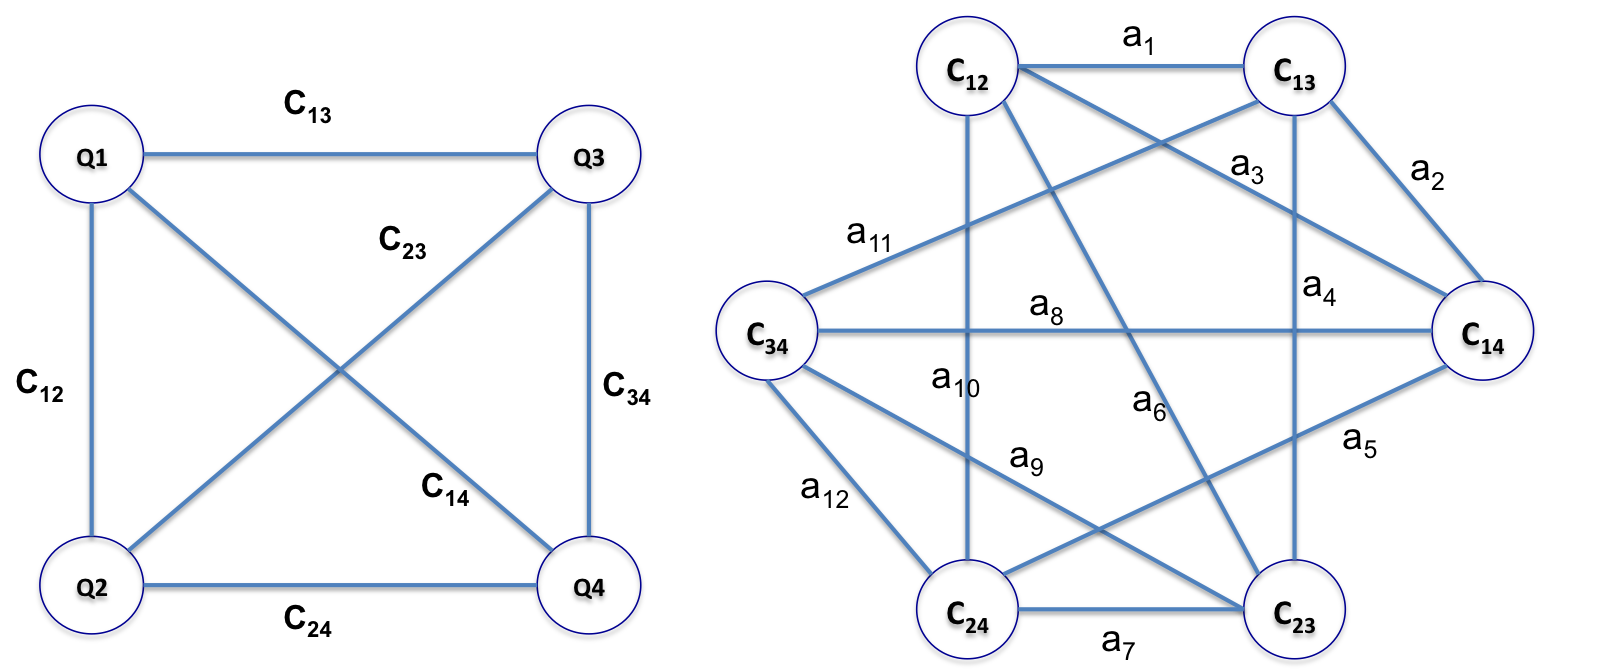
\includegraphics[scale=0.4]{constraintdual.png}
\caption{Left: constraint graph for the primal of the 4 Queens problem; Right: constraint graph for the dual of the 4 Queens problem}
\label{Figure 1}
\end{figure}


For the N Queen problem, we have $\frac{1}{2}n(n-1)$ constraints in the primal, which gives $\frac{1}{2}n(n-1)$ variables in the dual. The number of edges coming out from each vertex in the primal is same as the number of queens $n$. Therefore, we have $\frac{1}{4}n^2(n-1)$ edges for the dual of the constraint graph for the N queen problem (divide by 2 to remove duplicates since the edges are undirected).\\

For the N Queen problem, I tested the correctness of the CSP solver by solving for 4 Queens, 15 Queens and 20 Queens. The solution for 20-Queens is given as [1, 3, 5, 15, 11, 9, 2, 16, 18, 7, 10, 19, 17, 12, 20, 6, 8, 14, 4, 13], where the value of the $i^{th}$ entry denotes the row position of the queen in the $i^{th}$ column. We note that solving the 20-Queens problem using MAC3, MRV and LCV takes on average 0.15 seconds. 32 nodes are explored and 6916 constraints are checked. With just FC and MRV, the problem can be solved in even a shorter time period, taking on average 0.05 seconds, with 84 nodes explored and 2470 constraints checked. A more detailed discussion will be presented in Section 6.


\section{Sudoku}

For the Sudoku problem, I tested the correctness of the CSP solver by solving for the easy, medium and hard board. The solution for the hard board is given in Figure 2. In addition, I also run the bench mark test (short) for a combination of MAC3 or FC, MRV and LCV and the results are presented in Listing 9. I noted that the algorithm is the fastest for the CSP solver with FC and MRV, with an average run time of 0.33 seconds and maximum run time of 3.78 seconds. The hardest instance for all combinations happen to be the same sudoku puzzle. A more detailed discussion will be presented in Section 6.

\begin{figure}[H]
\centering
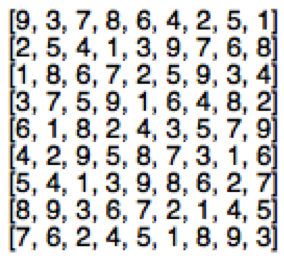
\includegraphics[scale=0.7]{sudoku.png}
\caption{Sudoku solution generated for hardBoard}
\label{Figure 1}
\end{figure}

\begin{lstlisting}[language=java,caption={results from benchmark test (short)}]
// MAC3, MRV, LCV
Running time: avg 0.98 max 10.12 variance 2.69
Explored nodes: avg 9037.34 max 115559 variance 265194159.30
Constraints checked: avg 1983068.56 max 22474702 variance 12420387676441.33
Hardest instance: 000000019800500000000000000300070500040000300000010000470000060000200400010900000
// FC, MRV, LCV
Running time: avg 0.35 max 4.03 variance 0.35
Explored nodes: avg 28601.93 max 343093 variance 2850252399.51
Constraints checked: avg 657456.38 max 7730340 variance 1453061295339.88
Hardest instance: 000000019800500000000000000300070500040000300000010000470000060000200400010900000
\end{lstlisting} 

\section{Circuit Board}

I also created the driver to solve for the circuit board layout problem. The variable is given as the coordinate of the lower left corner of the component. The domain of a variable corresponding to a component of width $w$ and height $h$, on a circuit board of width $n$ and height $m$ is given as the 2D integer coordinate space from $x=0$ to $x=n-w$ and $y=0$ to $y=m-h$. This will ensure that the component is able to fit within the board. The code is given in line 41 to 51 of the java file CircuitBoard.java.

\begin{lstlisting}[language=java,caption={48 legal pairs of locations for components a and b on 10x3 board}]
[(0,0)(3,0)],[(0,0)(4,0)],[(0,0)(5,0)],[(0,0)(3,1)],[(0,0)(4,1)],[(0,0)(5,1)],[(0,1)(3,0)],[(0,1)(4,0)],[(0,1)(5,0)],[(0,1)(3,1)],[(0,1)(4,1)],[(0,1)(5,1)],
[(1,0),(4,0)],[(1,0),(5,0)],[(1,0),(4,1)],[(1,0),(5,1)],[(1,1),(4,0)],[(1,1),(5,0)],[(1,1),(4,1)],[(1,1),(5,1)],
[(2,0),(5,0)],[(2,0),(5,1)],[(2,1),(5,0)],[(2,1),(5,1)],
[(5,0),(0,0)],[(5,0),(0,1)],[(5,1),(0,0)],[(5,1),(0,1)],
[(6,0),(0,0)],[(6,0),(0,1)],[(6,0),(1,0)],[(6,0),(1,1)],[(6,1),(0,0)],[(6,1),(0,1)],[(6,1),(1,0)],[(6,1),(1,1)],
[(7,0),(0,0)],[(7,0),(0,1)],[(7,0),(1,0)],[(7,0),(1,1)],[(7,0),(2,0)],[(7,0),(2,1)],[(7,1),(0,0)],[(7,1),(0,1)],[(7,1),(1,0)],[(7,1),(1,1)],[(7,1),(2,0)],[(7,1),(2,1)]
\end{lstlisting} 

We can also determine the constraints between two variables (it will be a pair of coordinates $[(i,j),(x,y)]$ where $(i,j)$ is the legal coordinate of the first component and $(x,y)$ is the legal coordinate of the second component. I give the explicit constraints for the components a and b on a 10x3 board in Listing 10 (there are 48 pairs). The basic idea is to have four nested loop to go through all possible comibination (code given in Listing 11). A function \verb`notOverlap` (code given in Listing 12) will check if a pair is legal by checking if the lower left, lower right, upper left and upper right of the second component fall within the area of the first component.

\begin{lstlisting}[language=java,caption={Create constraints}]
//preprocessing, refer to java file for detail
// code to get width and heights (w1,w2,h1,h2) of components, refer to java file for detail
// loop through all combinations
		for(int x1=0; x1<=boardWidth-w1; x1++){
			for(int y1=0; y1<=boardHeight-h1; y1++){
				for(int x2=0; x2<=boardWidth-w2; x2++){
					for(int y2=0; y2<=boardHeight-h2; y2++){
						if(notOverlap(x1,y1,w1,h1,x2,y2,w2,h2))
							constraint.add(new Pair<>(hashFunction(x1,y1),hashFunction(x2,y2)));
		// ...
		solver.addConstraint(components.get(i).index, components.get(j).index, constraint);
\end{lstlisting} 


\begin{lstlisting}[language=java,caption={notOverlap}]
    private boolean notOverlap(int x1, int y1, int w1, int h1, int x2, int y2, int w2, int h2){
        // check if the lower left of second is within the first
        if((x2>=x1) && (y2>=y1) && (x2<x1+w1) && (y2<y1+h1)) return false;
        // ...do the same : check if the lower right, upper left and upper right of the second is within the first, refer to java code for details
        return true; // otherwise
    }
\end{lstlisting} 


To convert the constraints/ domains into integer values for the generic CSP solver, I use a \verb`hashFunction` (refer to Java file for details) that basically convert a coordinate into an integer using $ x + y*maxSize$. \verb`maxSize` is a multiple of 10 constant and represents the largest dimension allowed. In my implementation, I set \verb`maxSize = 10000`.\\

I tested the CSP solver for the circuit board formulation on an easy board (the question given, 10x3 board for 4 components) and a harder board (10x10 board for 9 components). The output for the easy board is given in Figure 3 (Left) and the harder board is given in Figure 3 (Right). The former took 0.01 seconds to solve while the latter took 0.16 seconds, using MAC3 and MRV hueristic. More details will be presented in Section 6.

\begin{figure}[H]
\centering
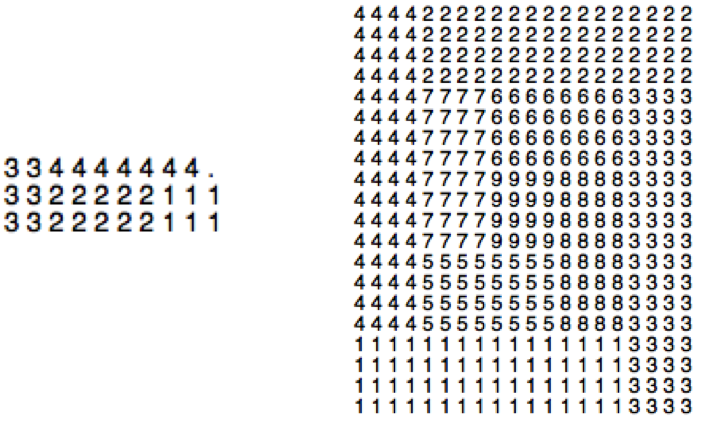
\includegraphics[scale=0.7]{circuit.png}
\caption{Left: Output of easy circuit board (question given); Right: Output of hard circuit board}
\label{Figure 2}
\end{figure}


\section{Experiment and Results}

I performed several experiments to measure the effectiveness of the various heuristics and inference techniques (MRV, LCV, FC, MAC-3) against the different kind of CSP problem (N Queens, Sudoku and Circuit Board layout). The results for runtime performance is given in Table 1, number of nodes explored is given in Table 2 and number of constraints checked is given in Table 3. An empty entry denotes that the runtime exceed 1 minute and is not recorded.\\

As we can observe from the table, FC with MRV has the fastest run time for the N-queen, sudoku and circuit board layout problem, followed by MAC-3 with MRV. It also seems like LCV, instead of speeding things up, actually slow things down. A possible explanation is the sorting algorithm used in \verb`orderDomainValues` introduced a \verb`nlog(n)` factor to the runtime, thus slowing things down. FC might be faster than MAC-3 because it tracks fewer nodes when checking for consistency. In addition, if there is an inconsistency caused by an assigned variable, usually it will be detected near the assigned variable instead of further away. It is interesting to note that the hard sudoku problem can only be solved within a minute when there is FC or MRV with MAC-3 heuristic involved. It is also interesting to note that the number of nodes explored is the least for FC+MRV. Again, FC and MRV reduces the number of node explored while LCV increases the number of nodes explored. The same relationship is observed for the number of constraints checked. Therefore, overall FC and MRV gives the greatest improvement in runtime.\\

\begin{table}[H]
\resizebox{\textwidth}{!}{%
\begin{tabular}{@{}rcccccccccc@{}}
\toprule
Run time (seconds)   & backtracking & MRV  & LCV  & MRV+LCV & FC   & FC+MRV+LCV & FC+MRV & MAC3 & MAC3+MRV+LCV & MAC3+MRV \\ \midrule
N Queen (4)          & 0            & 0    & 0.14 & 0.09      & 0    & 0.09          & 0        & 0    & 0.12            & 0          \\
N Queen (20)         & 4.03         & 5.13 & 6.87 & 7.26      & 2.09 & 0.28          & 0.05     & 5.2  & 0.22            & 0.18       \\
Sudoku (easy)        & 0.06         & 0.07 & 0.2  & 0.13      & 0.05 & 0.31          & 0.05     & 0.06 & 0.18            & 0.05       \\
Sudoku (hard)        & -            & -    & -    & -         & -    & 17.46         & 15       & -    & 48.33           & 46.81      \\
Circuit board (easy) & 0            & 0    & 0.17 & 0.13      & 0    & 0.1           & 0        & 0    & 0.2             & 0          \\
Circuit board (hard) & 0.1          & 0.09 & 0.25 & 0.22      & 0.08 & 0.18          & 0.06     & 0.21 & 0.48            & 0.11       \\ \bottomrule
\end{tabular}
}
\centering
\caption{Experiements performed to measure runtime with various heuristic}
\label{my-label}
\end{table}

\begin{table}[H]
\resizebox{\textwidth}{!}{%
\begin{tabular}{@{}rcccccccccc@{}}
\toprule
Nodes explored       & backtracking & MRV    & LCV    & MRV+LCV & FC    & FC+MRV+LCV & FC+MRV  & MAC3  & MAC3+MRV+LCV & MAC3+MRV \\ \midrule
N Queen (4)          & 9            & 9      & 9      & 9       & 7     & 7          & 7       & 5     & 5            & 5        \\
N Queen (20)         & 199636       & 199636 & 199636 & 199636  & 94405 & 85         & 84      & 10139 & 32           & 31       \\
Sudoku (easy)        & 82           & 82     & 82     & 82      & 82    & 82         & 82      & 82    & 82           & 82       \\
Sudoku (hard)        & -            & -      & -      & -       & -     & 1418065    & 1466690 & -     & 397980       & 411046   \\
Circuit board (easy) & 5            & 5      & 17     & 5       & 5     & 5          & 5       & 5     & 6            & 5        \\
Circuit board (hard) & 83           & 83     & 238    & 238     & 26    & 28         & 11      & 53    & 218          & 38       \\ \bottomrule
\end{tabular}
}
\centering
\caption{Experiements performed to measure number of nodes explored with various heuristic}
\label{my-label}
\end{table}

\begin{table}[H]
\resizebox{\textwidth}{!}{%
\begin{tabular}{@{}rcccccccccc@{}}
\toprule
Constraints checked  & backtracking & MRV      & LCV      & MRV+LCV  & FC      & FC+MRV+MRV & FC+MRV   & MAC3    & MAC3+MRV+LCV & MAC3+MRV \\ \midrule
N Queen (4)          & 62           & 62       & 57       & 57       & 36      & 36         & 36       & 58      & 58           & 58       \\
N Queen (20)         & 26660605     & 26660605 & 26660605 & 26660097 & 3079121 & 2470       & 2470     & 4431233 & 6916         & 7519     \\
Sudoku (easy)        & 8712         & 8712     & 8712     & 8712     & 8712    & 8712       & 8712     & 10322   & 10322        & 10322    \\
Sudoku (hard)        & -            & -        & -        & -        & -       & 32078076   & 33170936 & -       & 87632613     & 90879018 \\
Circuit board (easy) & 37           & 49       & 190      & 38       & 26      & 26         & 26       & 54      & 62           & 57       \\
Circuit board (hard) & 24440        & 24440    & 35236    & 35236    & 668     & 1812       & 348      & 4861    & 22073        & 3412     \\ \bottomrule
\end{tabular}
}
\centering
\caption{Experiements performed to measure number of constrainsts checked with various heuristic}
\label{my-label}
\end{table}

\section{Literature Review (Undergraduate student)}

I read the article written by Bessiere, Regin, Yap and Zhang on optimal coarse-grained arc consistency algorithm (Christian Bessière et al. “An optimal coarse-grained arc consistency algorithm”. In: Artificial Intelligence 165.2 (July 2005), pages 165–185.).\\

I learnt from the article that AC3 is a coarse-grained algorithm, as oppose to a fine-grained algorithm such as AC4. In a fine-grained algorithm, the removal of a value for a variable will influence the corresponding values in other variables while for a coarse-grained algorithm only influence the related variables. Coarse-grained algorithm has the advantage of being easy to implement with a constraint solver, however, its biggest disadvantage is that often time, it does not have an optimal worse case complexity unlike its fine-grained counterpart. Bessiere et al proposed a coarse-grained algorithm that has an optimal worse case complexity and is easy to intergrate with a constraint solver.\\

The primary reason for the sub-optimal worse case time complexity of AC3 is the line in the \verb`revise` function in which we always search from scratch if there exists a $(x,y)$ that does not satisfy the constraint. Bessiere et al idea is to only search from scratch the first time that line is called for a particular value and to store the information in a data structure that allows for constant look-up time, thus avoiding duplicate work. They proved the optimality of their algorithm mathematically (run time of $O(ed^2)$) and experimentally on the RLFAP and DOMINO CSP problem. This approach is interesting because again I see the trade-off between time complexity and space requirement.








\end{document}